\section*{Abstract}
\begin{textbf}


This study explores human-plant interaction within the Internet of Things paradigm. The Internet of Plants project tends to combine this paradigm with the will of getting closer to plants. Plants represent a full ecosystem of evolution, adaptation and communication. Thus, we are trying to enter their hidden world. Three plant species, Dypsis lutescens, Pachira glabra, and Dracaena, serve as conduits for inquiry, prompting participants to envisage a scenario where these botanical entities create and generate sounds upon physical interaction.

The methodology engages a diverse population of the engineering field including doctor and students. Participants imagine and interact with the envisaged musical plants, employing tactile approaches, namely Grasp, Pinch, Slide, Pet, and Tam Tam.

Findings highlight distinct interaction patterns influenced by plant characteristics, with users demonstrating nuanced responses to each species. The correlation between plant height and trunk interactions reveals environmental factors impacting human-plant dynamics. Additionally, interactions are categorized based on intensity, spatial displacement, and duration.

\end{textbf}

\begin{figure}[ht]
    \centering
    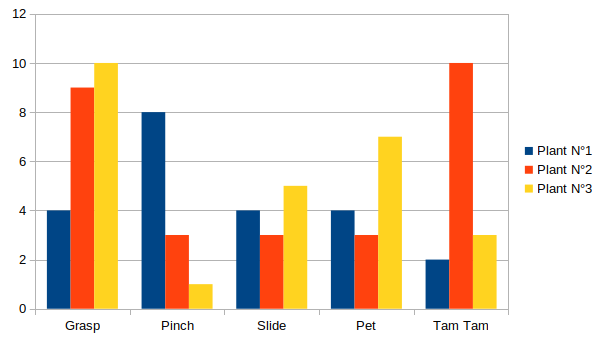
\includegraphics[width=0.42\textwidth]{Images/plant_interaction_chart.png}
    \caption{Bar chart that is extracting the main types of interaction regarding each plants.}
    
    \vspace{-0.5cm}
    \label{fig:setup_user_study}
    \vspace{0.2cm}
\end{figure}

\newpage